\begin{name}
	{Biên soạn \& Phản biện: Nhóm 4}
	{Cụm THPT Tỉnh Hưng Yên (Lần 1)}
\end{name}
\Opensolutionfile{ansbook}[ans/ansb\currfilebase]
\caulc
\Opensolutionfile{ans}[ans/ans\currfilebase-Phan-I]
\begin{ex}%[Dự án R8JJJF-VN-MT-15]%[2-KS-19-CumHungYen-L1-2026,TV034]%[1D1H4-8]
	Hằng ngày, mực nước của một con kênh lên xuống theo thuỷ triều. Độ sâu $h$ (m) của mực nước trong kênh tính theo thời gian $t$ (giờ) trong một ngày ($0\le t\le 24$) được cho bởi công thức $h(t) = 2\cos \left(\pi+\dfrac{\pi t}{6}\right)+12$. Độ sâu của mực nước tại thời điểm $t=3$\,giờ bằng
	\choice
		{$13$\,m}
		{$14$\,m}
		{\True $12$\,m}
		{$11$\,m}
	\loigiai{
		Tại thời điểm $t=3$\,giờ, ta có $h(3)=2\cos\left(\pi+\dfrac{\pi\cdot3}{6}\right)+12 = 12$ (m).
	}
\end{ex}

\begin{ex}%[Dự án 3PPWKF-VN-MT-15]%[2-KS-19-CumHungYen-L1-2026,TV034]%[2D4N1-2]
	Hàm số nào sau đây \textbf{không} là một nguyên hàm của hàm số $f(x)=3x^2+2x-1$?
	\choice
		{$F_1(x)=x^3+x^2-x$}
		{$F_2(x)=x^3+x^2-x+2\,026$}
		{\True $F_3(x)=x^3+x^2-1$}
		{$F_4(x)=x^3+x^2-x-1$}
	\loigiai{
		Họ nguyên hàm của hàm số $f(x)$ là
		\[\displaystyle\int f(x)\mathrm{\,d}x
		=\displaystyle\int\left(3x^2+2x-1\right)\mathrm{d}x
		=x^3+x^2-x+C,\ \text{với $C$ là hằng số}.\]
		Do đó $F_3(x)=x^3+x^2-1$ \textbf{không} là một nguyên hàm của hàm số $f(x)$.
	}
\end{ex}

\begin{ex}%[Dự án 62JTO3-VN-MT-15]%[2-KS-19-CumHungYen-L1-2026,TV034]%[2D4N2-1]
	Cho hàm số $f(x)$ liên tục trên $\mathbb{R}$ và hàm số $F(x)$ là nguyên hàm của hàm số $f(x)$. Biết $\displaystyle\int\limits_0^9 f(x)\mathrm{\,d}x=9$ và $F(0)=3$. Giá trị của $F(9)$ là
	\choice
		{$F(9)=-6$}
		{$F(9)=-12$}
		{$F(9)=6$}
		{\True $F(9)=12$}
	\loigiai{
		Ta có $\displaystyle\int\limits_0^9 f(x)\mathrm{\,d}x=9
		\Leftrightarrow F(9)-F(0)=9
		\Rightarrow F(9)=9+F(0)=9+3=12$.
	}
\end{ex}

\begin{ex}%[Dự án 1DMS8K-VN-MT-15]%[2-KS-19-CumHungYen-L1-2026,TV034]%[1H4N2-1]
	Cho hình chóp $S.ABC$. Khẳng định nào sau đây là đúng?
	\choice
		{$SA$ và $BC$ cắt và vuông góc với nhau}
		{$SA$ và $BC$ cắt nhau}
		{$SA$ và $BC$ song song với nhau}
		{\True $SA$ và $BC$ chéo nhau}
	\loigiai{
		\begin{center}
			\begin{tikzpicture}[scale=1, font=\footnotesize, line join=round, line cap=round, >=stealth]
    %hidden: VM005
				\path 
					(0,0) coordinate (A)
					+(0:4) coordinate (B)
					+(-45:3) coordinate (C)
					+(60:3.5) coordinate (S)
					;
				\draw[dashed] (A)--(B);
				\draw (A)--(C)--(B) (S)--(A) (S)--(B) (S)--(C);
				\foreach \p/\g in {A/180, B/0, C/-90, S/90} 
				{\fill (\p) circle (1pt) + (\g:2.5mm) node {$\p$};}
    \node at (0,0){\href{1DMS8K}{\tiny \phantom{1DMS8K}}};
			\end{tikzpicture}
		\end{center}
		Xét hình chóp $S.ABC$, ta có $SA$ và $BC$ không cùng nằm trong một mặt phẳng nên chúng chéo nhau.
	}
\end{ex}

\begin{ex}%[Dự án ZRN4QL-VN-MT-15]%[2-KS-19-CumHungYen-L1-2026,TV034]%[2H5N1-2]
	Trong không gian $Oxyz$, cho mặt phẳng $(\alpha)\colon 2x+4y-z+3=0$. Vectơ nào sau đây là một vectơ pháp tuyến của mặt phẳng $(\alpha)$?
	\choice
		{\True $\vec{n}_1=(2;4;-1)$}
		{$\vec{n}_3=(-2;4;1)$}
		{$\vec{n}_4=(2;4;1)$}
		{$\vec{n}_2=(2;-4;1)$}
	\loigiai{
		Từ phương trình mặt phẳng $(\alpha)\colon 2x+4y-z+3=0$, ta có một vectơ pháp tuyến của mặt phẳng $(\alpha)$ là $\vec{n}_1=(2;4;-1)$.
	}
\end{ex}

\begin{ex}%[Dự án 2C0Y1L-VN-MT-15]%[2-KS-19-CumHungYen-L1-2026,TV034]%[1D6H4-2]
	Phương trình $\log_3(x-1)=1$ có nghiệm là 
	\choice
		{\True $x=4$}
		{$x=1$}
		{$x=2$}
		{$x=3$}
	\loigiai{
		Điều kiện xác định $x-1>0\Leftrightarrow x>1$.\\
		Ta có $\log_3(x-1)=1\Leftrightarrow x-1=3\Leftrightarrow x=4$ (thoả mãn).\\
		Vậy phương trình $\log_3(x-1)=1$ có nghiệm là $x=4$.
	}
\end{ex}

\begin{ex}%[Dự án 5NH5WL-VN-MT-15]%[2-KS-19-CumHungYen-L1-2026,TV034]%[2H5H1-3]
	Trong không gian $Oxyz$, cho ba điểm $A(1;1;1)$, $B(0;2;1)$ và $C(1;-1;2)$. Mặt phẳng đi qua điểm $A$ và vuông góc với đường thẳng $BC$ có phương trình là 
	\choice
		{\True $x-3y+z+1=0$}
		{$x+3y+z-1=0$}
		{$x-3y+z-1=0$}
		{$x+3y-z+1=0$}
	\loigiai{
		Gọi $(P)$ là mặt phẳng đi qua điểm $A$ và vuông góc với đường thẳng $BC$.\\
		Khi đó, mặt phẳng $(P)$ là mặt phẳng đi qua điểm $A(1;1;1)$ và nhận $\overrightarrow{BC}=(1;-3;1)$ làm một vectơ pháp tuyến.\\
		Do đó, phương trình của mặt phẳng $(P)$ là 
		\[1(x-1)-3(y-1)+1(z-1)=0\Leftrightarrow x-3y+x+1=0.\]
	}
\end{ex}

\begin{ex}%[Dự án 1FEO4F-VN-MT-15]%[2-KS-19-CumHungYen-L1-2026,TV034]%[1D5H1-4]
	Khảo sát thời gian tập thể dục của một số học sinh khối $11$ thu được mẫu số liệu ghép nhóm sau:
	\begin{center}
		\begin{tabular}{|l|c|c|c|c|c|}
			\hline
			Thời gian (phút) & $[0;20)$ & $[20;40)$ & $[40;60)$ & $[60;80)$ & $[80;100)$\\
			\hline
			Số học sinh & $5$ & $9$ & $12$ & $10$ & $6$ \\
			\hline
		\end{tabular}
	\end{center} 
	Mốt của mẫu số liệu ghép nhóm trên bằng
	\choice
		{$53$}
		{\True $52$}
		{$54$}
		{$42$}
	\loigiai{
		Tần số lớn nhất là $12$ nên nhóm chứa mốt là nhóm $[40;60)$. \\
		Ta có $j=2$, $a_2=40$, $m_2=12$, $m_1=9$, $m_3=10$, $h=60-40=20$. Do đó
		\[M_{\text{o}}=40+\dfrac{12-9}{(12-9)+(12-10)}\cdot20=52.\]
	}
\end{ex}

\begin{ex}%[Dự án 2V7BHR-VN-MT-15]%[2-KS-19-CumHungYen-L1-2026,TV034]%[1D2H2-7]
	Giá của một chiếc xe ô tô lúc mới mua là $470$ triệu đồng. Trong $8$ năm đầu, cứ sau mỗi năm sử dụng, giá trị của chiếc xe ô tô giảm $40$ triệu đồng. Giá trị còn lại của xe sau $5$ năm sử dụng bằng
	\choice
		{$350$ triệu đồng}
		{$310$ triệu đồng}
		{\True $270$ triệu đồng}
		{$230$ triệu đồng}
	\loigiai{
		Gọi $(u_n)$ là giá trị của chiếc xe ô tô sau năm sử dụng thứ  $n$ ($1\le n\le8$) thì $(u_n)$ là một cấp số cộng có số hạng đầu $u_1=470-40=430$ và công sai $d=-40$.\\
		Giá trị còn lại của chiếc xe sau $5$ năm sử dụng ($n=5$) là 
		\[u_5=u_1+(5-1)\cdot d=430+4\cdot(-40)=270\  \text{(triệu đồng)}.\]
	}
\end{ex}

\begin{ex}%[Dự án 34TWWE-VN-MT-15]%[2-KS-19-CumHungYen-L1-2026,TV034]%[2H5H1-3]
	Trong không gian $Oxyz$, mặt phẳng $(P)$ cắt các trục $Ox$, $Oy$, $Oz$ lần lượt tại $A\left(\dfrac{14}{3};0;0\right)$, $B(0;7;0)$, $C(0;0;14)$. Phương trình mặt phẳng $(P)$ là 
	\choice
		{$2x+y+3z+9=0$}
		{\True $3x+2y+z-14=0$}
		{$2x+y+z-9=0$}
		{$3x+2y+z+14=0$}
	\loigiai{
		Mặt phẳng $(P)$ cắt các trục $Ox$, $Oy$, $Oz$ lần lượt tại $A\left(\dfrac{14}{3};0;0\right)$, $B(0;7;0)$, $C(0;0;14)$ nên có phương trình là 
		\[\dfrac{x}{\dfrac{14}{3}}+\dfrac{y}{7}+\dfrac{z}{14}=1\Leftrightarrow3x+2y+z-14=0.\]
	}
\end{ex}

\begin{ex}%[Dự án 5QC351-VN-MT-15]%[2-KS-19-CumHungYen-L1-2026,TV034]%[1H8H7-3]
	Cho hình hộp chữ nhật $ABCD.A'B'C'D'$ biết $AA'=4$, $AB=4$, $BC=6$. Thể tích khối chóp $A'.ABCD$ bằng 
	\choice
		{\True $32$}
		{$16$}
		{$96$}
		{$48$}
	\loigiai{
		\begin{center}
			\begin{tikzpicture}[scale=0.8, font=\footnotesize, line join=round, line cap=round, >=stealth]
    %hidden: VM005
				\path
					(0,0) coordinate (A)
					+(0:6) coordinate (D)
					+(-135:4) coordinate (B)
					($(B)+(D)-(A)$) coordinate (C)
					;
				\foreach \p in {A, B, C, D}
				{\path (\p)+(90:4) coordinate (\p');}
				\draw (D)--(C)--(B) (A')--(B')--(C')--(D')--cycle (B)--(B') (C)--(C') (D)--(D');
				\draw[dashed]  (A)--(A') (B)--(A)--(D);
				\foreach \p/\g in {A/150, B/-120, C/-60, D/0, A'/120, B'/180, C'/-20, D'/30}
				{\fill (\p) circle (1pt) + (\g:3mm) node {$\p$};}
    \node at (0,0){\href{5QC351}{\tiny \phantom{5QC351}}};
			\end{tikzpicture}
		\end{center}
		Vì $ABCD.A'B'C'D'$ là hình hộp chữ nhật nên $AA'\perp (ABCD)$ và $S_{ABCD}=AB\cdot BC=4\cdot6=24$.\\
		Do đó, thể tích của khối chóp $A'.ABCD$ là $V=\dfrac{1}{3}\cdot S_{ABCD}\cdot AA'
		=\dfrac{1}{3}\cdot 24\cdot 4=32$.
	}
\end{ex}

\begin{ex}%[Dự án 1SUFTC-VN-MT-15]%[2-KS-19-CumHungYen-L1-2026,TV034]%[2D1N2-2]
	Cho hàm số $y=f(x)$ xác định trên $\mathbb{R}$ và có bảng biến thiên sau:
	\begin{center}
		\begin{tikzpicture}
    %hidden: VM005
			\tkzTabInit[nocadre=true, lgt=1, espcl=3.5, deltacl=0.5]
			{$x$/0.7,$y’$/0.7,$y$/2}
			{$-\infty$,$-7$,$-4$,$+\infty$}
			\tkzTabLine{,-,0,+,0,-,}
			\tkzTabVar{+/$+\infty$,-/$-6$,+/$-3$,-/$-\infty$}
    \node at (T11){\href{1SUFTC}{\tiny \phantom{1SUFTC}}};
		\end{tikzpicture}
	\end{center}
	Điểm cực đại của hàm số $y=f(x)$ là
	\choice
		{$x=-3$}
		{\True $x=-4$}
		{$x=-7$}
		{$x=-6$}
	\loigiai{
		Từ bảng biến thiên, ta có điểm cực đại của hàm số $y=f(x)$ là $x=-4$.
	}
\end{ex}

\Closesolutionfile{ans}
\cauds
\Opensolutionfile{ans}[ans/ans\currfilebase-Phan-II]
\begin{ex}%[Dự án 2OXG48-VN-MT-15]%[2-KS-19-CumHungYen-L1-2026,TV025]%[2H2V2-6]
	Một kho chứa hàng có dạng hình lăng trụ đứng $OAFPE.CBGQH$ với $OAFE$ là hình chữ nhật và $EPF$ là tam giác cân tại $P$. 
	Biết $OA=4$\,m; $AB=6$\,m; $HC=5$\,m; độ dốc của mái nhà, tức là số đo góc phẳng nhị diện $[Q,FG,H]$ bằng $45^\circ$. Người ta mô hình hóa nhà kho bằng cách chọn hệ trục toạ độ tương ứng như hình vẽ sau đây (đơn vị trên mỗi trục là $1$\,m).
	\begin{center}
		\begin{tikzpicture}[scale=1, font=\footnotesize, line join=round, line cap=round, >=stealth]
    %hidden: VM005
			\path 
				(0,0) coordinate (O) node[below left]{$O$}
				(4,0) coordinate (A) node[below]{$A$}
				(0,3) coordinate (E) node[left]{$E$}
				($(A)+(E)-(O)$) coordinate (F)node[right]{$F$}
				(A)+(1,2) coordinate (B) node[right]{$B$}
				($(O)+(B)-(A)$) coordinate (C) node[left]{$C$}
				($(C)+(E)-(O)$) coordinate (H) node[left]{$H$}
				($(H)+(B)-(C)$) coordinate (G) node [right]{$G$}
				($(O)!.5!(A)$) coordinate (x)
				(x)+(0,4.5) coordinate (P) node[below]{$P$}
				($(P)+(H)-(E)$) coordinate (Q) node[above]{$Q$}
				;
			\draw[->] (O)--(E)--($(E)+(90:1)$)node[left]{$z$};
			\draw[->] (O)--(A)--($(A)+(0:1)$) node[below]{$x$};
			\draw[dashed,->] (O)--(C)--($(O)!1.3!(C)$) node[right]{$y$};
			\draw (A)--(B)--(G)--(Q)--(H)--(E)--(F)--cycle (E)--(P)--(F) (P)--(Q) (F)--(G);
			\draw[dashed] (C)--(B) (C)--(H)--(G);
			\foreach \t in {A,B,C,O,E,F,G,H,P,Q}{
			\fill (\t) circle (1pt);
			}
    \node at (0,0){\href{2OXG48}{\tiny \phantom{2OXG48}}};
		\end{tikzpicture} 
	\end{center}
	\choiceTF
		{Tọa độ của điểm $G$ là $(6;4;5)$}
		{\True Tọa độ của $\overrightarrow{PQ}$ là $(0;6;0)$}
		{\True Chiều cao kho hàng tức là khoảng cách từ nóc nhà (điểm cao nhất của nóc nhà) và sàn nhà bằng $7$ (m)}
		{\True Người ta muốn lắp camera quan sát trong nhà kho tại vị trí trung điểm $M$ của đoạn thẳng $GQ$ và đầu thu dữ liệu đặt tại vị trí $O$. Người ta thiết kế đường dây cáp nối từ đầu thu dữ liệu $O$ đến camera. Biết rằng đường dây cáp đi qua điểm $E$ và điểm $H$. Độ dài đoạn cáp nối tối thiểu để kết nối đầu thu với camera bằng $11+\sqrt{10}$ (m)}
	\loigiai{
		\begin{center}
			\begin{tikzpicture}[scale=1, font=\footnotesize, line join=round, line cap=round, >=stealth]
    %hidden: VM005
				\path 
					(0,0) coordinate (O) node[below left]{$O$}
					(4,0) coordinate (A) node[below]{$A$}
					(0,3) coordinate (E) node[left]{$E$}
					($(A)+(E)-(O)$) coordinate (F) node[right]{$F$}
					(A)+(1,2) coordinate (B) node[right]{$B$}
					($(O)+(B)-(A)$) coordinate (C) node[left]{$C$}
					($(C)+(E)-(O)$) coordinate (H) node[left]{$H$}
					($(H)+(B)-(C)$) coordinate (G) node [right]{$G$}
					($(O)!.5!(A)$) coordinate (x)
					(x)+(0,4.5) coordinate (P) node[right]{$P$}
					($(P)+(H)-(E)$) coordinate (Q) node[above]{$Q$}
					($(E)!0.5!(F)$) coordinate (I)
					($(Q)!0.5!(G)$) coordinate (M)
					;
				\draw[->] (O)--(E)--($(E)+(90:1)$) node[left]{$z$};
				\draw[->] (O)--(A)--($(A)+(0:1)$) node[below]{$x$};
				\draw[dashed,->] (O)--(C)--($(O)!1.3!(C)$) node[right]{$y$} ;
				\draw (A)--(B)--(G)--(Q)--(H)--(E)--(F)--cycle (E)--(P)--(F) (P)--(Q) (F)--(G)
					(P)--(I) node[below] {$I$}
					;
				\draw[dashed] (C)--(B) (C)--(H)--(G)
					(H)--(M) node[above right]{$M$}
					;
				\foreach \t in {A,B,C,O,E,F,G,H,P,Q,M,I}
				{\fill (\t) circle (1pt);}
    \node at (0,0){\href{2OXG48}{\tiny \phantom{2OXG48}}};
			\end{tikzpicture}
		\end{center}
		\begin{itemchoice}
			\itemch Ta có $A(4;0;0)$, $B(4;6;0)$, $C(0;6;0)$, $H(0;6;5)$.\\
			Suy ra $G(4;6;5)$.
			\itemch Do nhà kho $OAFPE.CBGQH$ có dạng hình lăng trụ đứng nên $\overrightarrow{PQ}=\overrightarrow{OC}=(0;6;0)$.
			\itemch Gọi $I$ là trung điểm của $EF$.\\
			Khi đó $PI$ là đường trung tuyến trong $\triangle EPF$ vuông cân tại $P$ nên \[PI = \dfrac{1}{2} EF = \dfrac{1}{2} \cdot 4 = 2\ \text{(m)}.\]
			Suy ra $PI + FA = 2 + 5 = 7$ (m).\\
			Vậy khoảng cách giữa nóc nhà và sàn nhà là $7$\,m.
			\itemch 
			Ta có $FG \perp (CBGQH)$ (vì $OAFPE.CBGQH$ là hình lăng trụ đứng).\\
			Suy ra $QG \perp FG$, $HG \perp FG$ nên số đo góc phẳng nhị diện $[Q,FG,H]$ là 
			$\widehat{QGH} = 45^\circ$.\\
			Do đó $\triangle EPF$ là tam giác vuông cân tại $P$, suy ra $\triangle HQG$ cũng là tam giác vuông cân tại $Q$.\\
			Khi đó, ta có $QH=QG=\dfrac{HG}{\sqrt{2}}=\dfrac{4}{\sqrt{2}}=2\sqrt{2}$ (m).\\
			Gọi $M$ là trung điểm của $QG$ suy ra $QM=\sqrt{2}$ (m).\\
			Xét $\triangle QHM$ vuông tại $Q$ có $HM^2=QM^2+QH^2$.\\
			Suy ra $HM=\sqrt{\left(\sqrt{2}\right)^2+\left(2\sqrt{2}\right)^2}=\sqrt{10}$ (m).\\
			Vậy độ dài đoạn cáp nối tối thiểu là $OE+EH+HM=5+6+\sqrt{10}=11+\sqrt{10}$ (m).
		\end{itemchoice}
	}
\end{ex}

\begin{ex}%[Dự án 18XOVR-VN-MT-15]%[2-KS-19-CumHungYen-L1-2026,TV025]%[2D3H2-3]
	Điểm trung bình môn Toán cuối năm của các học sinh lớp $12$A và $12$B được thống kê ở bảng sau.
	\begin{center}
		\begin{tabular}{|c|c|c|c|c|c|}
			\hline
			Điểm trung bình & $[5;6)$ & $[6;7)$ & $[7;8)$ & $[8;9)$ &$[9;10)$\\
			\hline
			$12$A & $1$ & $0$ & $11$ & $22$ &$6$\\
			\hline
			$12$B & $0$ & $6$ & $8$ & $14$ & $12$\\
			\hline
		\end{tabular}
	\end{center}
	\choiceTF
		{\True Lớp $12$A có $28$ học sinh có điểm trung bình môn Toán cuối năm từ $8$ trở lên}
		{Số trung bình của mẫu số liệu lớp $12$A lớn hơn số trung bình của mẫu số liệu lớp $12$B}
		{Độ lệch chuẩn của mẫu số liệu lớp $12$A (làm tròn kết quả đến hàng phần trăm) là $0{,}72$}
		{\True Nếu so sánh theo độ lệch chuẩn thì học sinh lớp $12$A có điểm trung bình môn Toán cuối năm ít phân tán hơn lớp $12$B}
	\loigiai{	\begin{center}
			\begin{tabular}{|c|c|c|c|c|c|}
				\hline
				Điểm trung bình & $[5;6)$ & $[6;7)$ & $[7;8)$ & $[8;9)$ &$[9;10)$\\
				\hline
				Giá trị đại diện & $5{,}5$ & $6{,}5$ & $7{,}5$ & $8{,}5$ &$9{,}5$\\
				\hline
				$12$A & $1$ & $0$ & $11$ & $22$ &$6$\\
				\hline
				$12$B & $0$ & $6$ & $8$ & $14$ & $12$\\
				\hline
			\end{tabular}
		\end{center}
		\begin{itemchoice}
			\itemch Từ bảng thống kê ta thấy số học sinh có số điểm trung bình môn Toán từ $8$ trở lên của lớp $12$A là $22+6=28$ học sinh.
			\itemch 
			Số trung bình môn Toán của lớp $12$A là
			$$\overline{x}_A=\dfrac{1\cdot5{,}5+0\cdot6{,}5+11\cdot7{,}5+22\cdot8{,}5+6\cdot 9{,}5}{40}=8{,}3.$$
			Số trung bình môn Toán của lớp $12$B là
			$$\overline{x}_B=\dfrac{0\cdot5{,}5+6\cdot6{,}5+8\cdot7{,}5+14\cdot8{,}5+12\cdot 9{,}5}{40}=8{,}3.$$
			Vậy số trung bình của mẫu số liệu lớp $12$A bằng số trung bình của mẫu số liệu lớp $12$B.
			\itemch 
			Phương sai của mẫu số liệu ghép nhóm điểm môn Toán của lớp $12$A là
			$$s_A^2=\dfrac{1\cdot5{,}5^2+0\cdot6{,}5^2+11\cdot7{,}5^2+22\cdot8{,}5^2+6\cdot 9{,}5^2}{40}-8{,}3^2=0{,}61.$$
			Do đó độ lệch chuẩn $s_A\approx0{,}78$.
			\itemch
			Phương sai của mẫu số liệu ghép nhóm điểm môn Toán của lớp $12$B là
			$$s_B^2=\dfrac{0\cdot5{,}5^2+6\cdot6{,}5^2+8\cdot7{,}5^2+14\cdot8{,}5^2+12\cdot 9{,}5^2}{40}-8{,}3^2=1{,}06.$$
			Do đó, ta được độ lệch chuẩn $s_B\approx1{,}03$.\\
			Vì $s_A <s_B$ nên  học sinh lớp $12$A có điểm trung bình môn Toán cuối năm ít phân tán hơn lớp $12$B.
		\end{itemchoice}
	}
\end{ex}

\begin{ex}%[Dự án 1RXS1R-VN-MT-15]%[2-KS-19-CumHungYen-L1-2026,TV028]%[2D1H3-1]
	Cho hàm số $y = f(x) = \left(x^2 - 5x + 7\right)\mathrm{e}^x$.
	\choiceTF
		{\True $f(0) = 7$}
		{Đạo hàm của hàm số đã cho là $f'(x) = (2x - 5)\mathrm{e}^x$}
		{\True Giá trị nhỏ nhất và lớn nhất của hàm số $y = f(x)$ trên đoạn $[0; 2]$ lần lượt là $7$ và $3\mathrm{e}$}
		{Hàm số $y = f(x)$ nghịch biến trên khoảng $\left(-\infty; \dfrac{5}{2}\right)$ và đồng biến trên khoảng $\left(\dfrac{5}{2}; +\infty\right)$}
	\loigiai{
		Xét hàm số $y = f(x) = (x^2 - 5x + 7)\mathrm{e}^x$.
		\begin{itemchoice}
			\itemch Ta có 
			$f(0) = \left(0^2-5\cdot 0+7\right)\mathrm{e}^0=7$.
			\itemch Ta có 
			$f'(x) = (2x - 5)\mathrm{e}^x + (x^2 - 5x + 7)\mathrm{e}^x = (x^2 - 3x + 2)\mathrm{e}^x$.
			\itemch Phương trình $f'(x) = 0 \Leftrightarrow (x^2 - 3x + 2)\mathrm{e}^x =0 \Leftrightarrow x^2 - 3x + 2=0 \Leftrightarrow \hoac{&x=1\in [0;2]\\&x=2\in [0;2].}$\\
			Ta có $f(0) = 7$; $f(1) = 3\mathrm{e}$; $f(2) = \mathrm{e}^2$.\\
			So sánh các giá trị, ta được $7 < \mathrm{e}^2 < 3\mathrm{e}$.\\
			Vậy trên đoạn $[0; 2]$, hàm số $y=f(x)$ có giá trị nhỏ nhất là $7$ và có giá trị lớn nhất là $3\mathrm{e}$.
			\itemch 
			Bảng biến thiên
			\begin{center}
				\begin{tikzpicture}
    %hidden: VM005
					\tkzTabInit[nocadre=true, lgt=1.2, espcl=3, deltacl=0.5]
					{$x$/0.7,$f’(x)$/0.7,$f(x)$/2}
					{$-\infty$, $1$, $2$, $+\infty$}
					\tkzTabLine{,+,0,-,0,+,}
					\tkzTabVar{-/ $-\infty$, +/ $3\mathrm{e}$, -/ $\mathrm{e}^2$, +/ $+\infty$}
    \node at (T11){\href{1RXS1R}{\tiny \phantom{1RXS1R}}};
				\end{tikzpicture}
			\end{center}
			Dựa vào bảng biến thiên, ta thấy hàm số đồng biến trên các khoảng $(-\infty; 1)$ và $(2; +\infty)$, nghịch biến trên khoảng $(1; 2)$.
		\end{itemchoice}
	}
\end{ex}

\begin{ex}%[Dự án 5TZ03X-VN-MT-15]%[2-KS-19-CumHungYen-L1-2026,TV028]%[2D4V3-1]
	\immini[thm]{Cho hàm số $y = f(x)$ xác định trên $\mathbb{R}$, có nguyên hàm trên $\mathbb{R}$ là hàm số $y = F(x)$. Hàm số $y = f(x)$ có đồ thị như hình vẽ bên. Biết $F(4) = 7$ và diện tích hai phần gạch chéo $S_1$; $S_2$ lần lượt là $8$; $20$.		\choiceTF
		{\True $\displaystyle \int \limits_{-1}^{1} f(x) \mathrm{\,d}x = 8$}
		{\True $\displaystyle \int \limits_{-1}^{4} \big|f(x)\big| \mathrm{d}x = 28$}
		{$\displaystyle \int \limits_{-1}^{4} f(x) \mathrm{\,d}x = 28$}
		{\True $3F(1) - 7F(-1) = -52$}
		}
			{
			\begin{tikzpicture}[scale=0.7, font=\footnotesize, line join=round,
    %hidden: VM005
				line cap=round, >=stealth]
				\def\f{0.5*(\x+1)*(\x-1)*(\x-4)}
				\fill[pattern=north east lines, pattern color=violet!70,opacity=0.4] (-1,0) -- plot[domain=-1:1, smooth] (\x,{\f}) -- (1,0) -- cycle;
				\fill[pattern=north east lines, pattern color=violet!70,opacity=0.4] (1,0) -- plot[domain=1:4, smooth] (\x,{\f}) -- (4,0) -- cycle;
				\draw[->] (-2.5,0) -- (5.5,0) node[below] {$x$};
				\draw[->] (0,-4.5) -- (0,3) node[left] {$y$};
				\draw[domain=-1.61:4.33, smooth, samples=100] plot (\x,{\f});
				\node[below left] at (-1,0) {$-1$};
				\node[below left] at (1,0) {$1$};
				\node[below right] at (4,0) {$4$};
				\node at (-0.3, 0.7) {$S_1$};
				\node at (2.5, -1.5) {$S_2$};
				\fill (-1,0) circle(1pt) (1,0) circle(1pt) (4,0) circle(1pt) (0,0) node[below left]{$O$} circle(1pt);
    \node at (0,0){\href{5TZ03X}{\tiny \phantom{5TZ03X}}};
			\end{tikzpicture}
			}	
	\loigiai{
		\begin{itemchoice}
			\itemch Dựa vào đồ thị, ta thấy hàm số $f(x) \ge 0$, $\forall x \in [-1; 1]$ nên \[\displaystyle \int \limits_{-1}^{1} \big|f(x)\big| \mathrm{d}x
			= \displaystyle \int \limits_{-1}^{1} f(x) \mathrm{\,d}x = S_1 = 8.\]
			\itemch Ta có $\displaystyle \int \limits_{-1}^{4} \big|f(x)\big| \mathrm{d}x =\displaystyle \int \limits_{-1}^{1} \big|f(x)\big| \mathrm{d}x+\displaystyle \int \limits_{1}^{4} \big|f(x)\big| \mathrm{d}x = S_1 + S_2 = 8 + 20 = 28$.
			\itemch Dựa vào đồ thị, ta thấy hàm số $f(x) \le 0$, $\forall x \in [1; 4]$ nên \[\displaystyle \int \limits_{1}^{4} \big|f(x)\big| \mathrm{d}x = - \displaystyle \int \limits_{1}^{4} f(x) \mathrm{\,d}x = S_2 = 20 \Rightarrow \displaystyle \int \limits_{1}^{4} f(x) \mathrm{\,d}x = -20.\]
			Do đó $\displaystyle \int \limits_{-1}^{4} f(x) \mathrm{\,d}x = \displaystyle \int \limits_{-1}^{1} f(x) \mathrm{\,d}x + \displaystyle \int \limits_{1}^{4} f(x) \mathrm{\,d}x = 8 + (-20) = -12$.
			\itemch Ta có $\displaystyle \int \limits_{1}^{4} f(x) \mathrm{\,d}x = F(4) - F(1) = -20$.\\
			Mà $F(4) = 7$ nên $7 - F(1) = -20 \Leftrightarrow F(1) = 27$.\\
			Lại có $\displaystyle \int \limits_{-1}^{1} f(x) \mathrm{\,d}x = F(1) - F(-1) = 8$.\\
			Suy ra $27 - F(-1) = 8 \Leftrightarrow F(-1) = 19$.\\
			Do đó $3F(1) - 7F(-1) = 3 \cdot 27 - 7 \cdot 19 = -52$.
		\end{itemchoice}
	}
\end{ex}

\Closesolutionfile{ans}
\caukq
\Opensolutionfile{ans}[ans/ans\currfilebase-Phan-III]
\begin{ex}%[Dự án 65HJJ7-VN-MT-15]%[2-KS-19-CumHungYen-L1-2026,TV019]%[2D1H1-5]
	Sau khi phát hiện một bệnh dịch, các chuyên gia y tế ước tính số người nhiễm bệnh kể từ ngày xuất hiện bệnh nhân đầu tiên đến ngày thứ $t$ là $f(t) = 45t^2 - t^3$, $t=0$, $1$, $2$, $\ldots$, $25$. Nếu coi $f(t)$ là hàm số xác định trên đoạn $[0;25]$ thì đạo hàm $f'(t)$ được xem là tốc độ truyền bệnh (người/ngày) tại thời điểm $t$. Giả sử khoảng thời gian mà tốc độ truyền bệnh giảm là từ ngày thứ $m$ đến ngày thứ $n$. Khi đó, giá trị $n - m$ bằng bao nhiêu?
	\par\shortans{$10$}
	\loigiai{
		Tốc độ truyền bệnh tại thời điểm $t$ là
		\[v(t)=f'(t)=90t-3t^2,\ \text{với }t\in[0;25].\]
		Đạo hàm $v'(t)=90-6t=0\Leftrightarrow t=15$.\\
		Bảng biến thiên
		\begin{center}
			\begin{tikzpicture}
    %hidden: VM005
				\tkzTabInit[nocadre=true,lgt=1.2,espcl=4,deltacl=0.5]
				{$t$/0.7,$v’(t)$/0.7,$v(t)$/2}
				{$0$, $15$, $25$}
				\tkzTabLine{,+, 0,- ,} 
				\tkzTabVar{-/$0$, +/$675$, -/$375$}
    \node at (T11){\href{65HJJ7}{\tiny \phantom{65HJJ7}}};
			\end{tikzpicture}
		\end{center}
		Dựa vào bảng biến thiên, ta thấy hàm số $v(t)$ nghịch biến trong khoảng $(15;25)$, tức là tốc độ truyền bệnh giảm từ ngày thứ $15$ đến ngày thứ $25$.\\
		Do đó $\,m = 15$ và $n = 25$.\\
		Vậy $n - m = 25 - 15 = 10$.
	}
\end{ex}

\begin{ex}%[Dự án 4O4XKK-VN-MT-15]%[2-KS-19-CumHungYen-L1-2026,TV019]%[2D1V3-6]
	Một công ty tiến hành khai thác $15$ giếng dầu trong khu vực được chỉ định. Trung bình mỗi giếng dầu chiết xuất được $231$ thùng dầu mỗi ngày. Công ty có thể khai thác nhiều hơn $15$ giếng dầu nhưng cứ khai thác thêm một giếng thì lượng dầu mỗi giếng chiết xuất được hằng ngày sẽ giảm $7$ thùng. Để giám đốc công ty có thể quyết định số giếng cần thêm cho phù hợp, hãy chỉ ra số giếng công ty khai thác thêm để sản lượng dầu chiết xuất được là lớn nhất.
	\par\shortans{$9$}
	\loigiai{
		Gọi $x$ là số giếng dầu công ty khai thác thêm ($x\in\mathbb{N}^*$).\\
		Khi đó, tổng số giếng dầu khai thác là $15+x$ (giếng).\\
		Sản lượng dầu chiết xuất được của mỗi giếng trong một ngày là $231 - 7x$ (thùng).\\
		Điều kiện $231-7x>0\Leftrightarrow x<33$ hay $x\in(0;33)$.\\
		Tổng sản lượng dầu chiết xuất được mỗi ngày của công ty là
		\[P(x)=(15+x)(231-7x)=-7x^2+126x+3\,465.\]
		Xét hàm số $P(x)=-7x^2+126x+3\,465$, $\forall x\in(0;33)$.\\
		Ta có $P'(x)=-14x+126$.\\
		Phương trình $P'(x)=0\Leftrightarrow-14x+126=0\Leftrightarrow x=9\in(0;33)$.\\
		Bảng biến thiên
		\begin{center}
			\begin{tikzpicture}
    %hidden: VM005
				\tkzTabInit[nocadre=true, lgt=1.2, espcl=4, deltacl=0.6]
				{$x$/0.7,$P'(x)$/0.7,$P(x)$/2}
				{$0$, $9$,$33$}
				\tkzTabLine{,+,0,-,}
				\tkzTabVar{-/$3\,465$,+/$4\,032$,-/$0$}
    \node at (T11){\href{4O4XKK}{\tiny \phantom{4O4XKK}}};
			\end{tikzpicture}
		\end{center}
		Vậy công ty cần khai thác thêm $9$ giếng dầu để tổng sản lượng dầu chiết xuất được là lớn nhất.
	}
\end{ex}

\begin{ex}%[Dự án QOBXDF-VN-MT-15]%[2-KS-19-CumHungYen-L1-2026,TV030]%[2D4V3-5]
	Một thùng làm kem có dạng khối tròn xoay, có mặt cắt qua trục là dạng parabol như hình vẽ. Biết phương trình nửa đường biên parabol bên trái có dạng $f(x) = a\sqrt{x}$. Hỏi dung tích của thùng làm kem bằng bao nhiêu lít (làm tròn kết quả đến hàng phần mười)?
	\begin{center}
		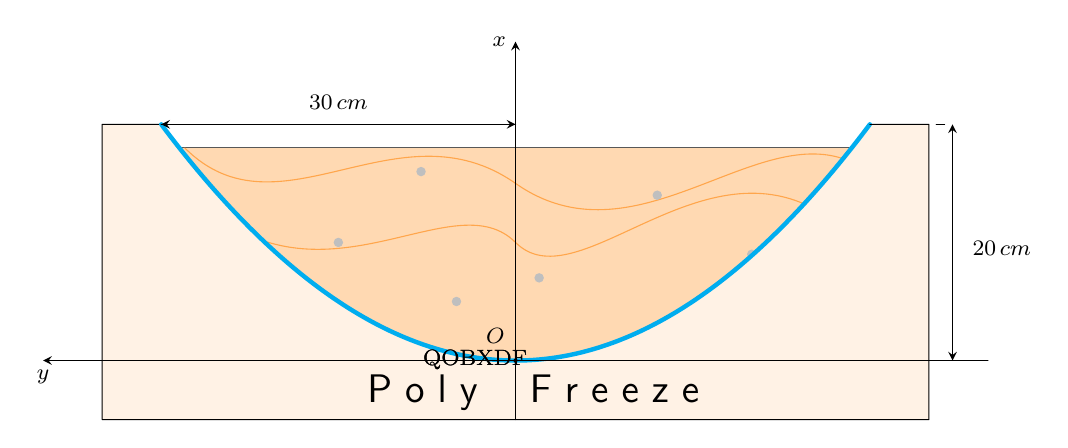
\begin{tikzpicture}[scale=0.15, font=\footnotesize, line join=round,
    %hidden: VM005
			line cap=round, >=stealth]
			% Vẽ khối màu kem (Poly Freeze) làm nền
			\filldraw[fill=orange!10, draw=black] (-30,20) -- (-35,20) -- (-35,-5) -- (35,-5)--(35,20)--(30,20)--(28.5,18)--(-28.5,18)--cycle;
			\begin{scope}
				% Clip miền giới hạn bởi parabol x = y^2/45
				\clip plot[domain=-30:30] (\x, {(\x)^2/45}) -- cycle;
				% Tô màu nền chất lỏng
				\fill[orange!30] (-30,0) rectangle (30,18);
				% Vẽ các đường sóng sánh ngẫu nhiên (Bezier curves)
				\draw[orange!70] 
					(-28,18) .. controls (-20,10) and (-10,22) .. (0,15)
					.. controls (10,8) and (20,20) .. (28,17);
				\draw[orange!70]
					(-25,12) .. controls (-15,5) and (-5,15) .. (0,10)
					.. controls (5,5) and (15,18) .. (25,13);
				% giống đá vụn
				\foreach \p in {(-15,10), (-8,16), (2,7), (12,14), (20,9), (-5,5)}
				\fill[gray!50] \p circle (0.4);
			\end{scope}
			% Vẽ đường cong màu xanh ngọc (Parabol) đậm
			\draw[cyan, ultra thick, smooth, samples=100, domain=-30:30] 
				plot(\x, {(\x)^2/45});
			%  Vẽ hệ trục tọa độ xOy
			\draw[->] (40,0) -- (-40,0) node[below] {$y$};
			\draw[->] (0,-5) -- (0,27) node[left] {$x$};
			% Đường 30 cm (bán kính)
			\draw[dashed, thin] (0,20) -- (-30,20);
			\draw[<->] (0,20) -- (-30,20);
			\fill (-15,20.2)  node[shift=(90:0.25)]{$30\,\text{cm}$};
			% Đường 20 cm (chiều cao)
			\draw[dashed] (30,20) -- (37,20);
			\draw[dashed] (30,0) -- (35,0);
			\draw[<->] (37,0) -- (37,20) ;
			\fill (39.5,9.5)  node[shift=(0:0.25)]{$20\,\text{cm}$};
			\fill (0,0) node{\href{QOBXDF}{\tiny \phantom{QOBXDF}}} circle (5pt)  node[shift=(130:0.4)]{$O$};
			% Chữ Poly Freeze
			\node[font=\Large\sffamily] at (1.5,-2.7) {P o l y \quad F r e e z e};
    \node at (0,0){\href{QOBXDF}{\tiny \phantom{QOBXDF}}};
		\end{tikzpicture}
	\end{center}
	\par
	\shortans{$28{,}3$}
	\loigiai{
		Gắn hệ trục toạ độ $Oxy$ như hình vẽ sau:
		\begin{center}
			\begin{tikzpicture}[scale=1, font=\footnotesize, line join=round,
    %hidden: VM005
				line cap=round, >=stealth]
				\def \xmin{-1}
				\def \xmax{3}
				\def \ymin{-3.5}
				\def \ymax{4}
				\draw[->] (\xmin,0)--(\xmax,0) node[below] {$x$};
				\draw[->] (0,\ymin)--(0,\ymax) node[left] {$y$};
				\fill (0,0) node{\href{QOBXDF}{\tiny \phantom{QOBXDF}}} circle(1pt) node[below left]{$O$}
					(2,0) circle(1pt) node[shift=(-45:0.4)]{$20$}
					(0,3) circle(1pt) node[shift=(180:0.3)]{$30$}
					(0,-3) circle(1pt) node[shift=(180:0.5)]{$-30$}
					(2,3) circle(1pt) (2,-3) circle(1pt)
					;
				\draw[dashed] (0,3)--(2,3)--(2,-3)--(0,-3);
				\clip (\xmin,-3) rectangle (\xmax,3);
				\draw[smooth, samples=100, domain=0:4.5] 
					plot(\x, {2.121*sqrt(\x)});
				\draw[smooth, samples=100, domain=0:4.5] 
					plot(\x, {-2.121*sqrt(\x)});
    \node at (0,0){\href{QOBXDF}{\tiny \phantom{QOBXDF}}};
			\end{tikzpicture}
		\end{center}
		Đường biên parabol bên trái $f(x)=a\sqrt{x}$ đi qua điểm có toạ độ $(20;30)$ nên
		\[a\sqrt{20} = 30 \Rightarrow a = 3\sqrt{5}.\]
		Suy ra $f(x)=3\sqrt{5}\cdot\sqrt{x}$.\\
		Dung tích của thùng làm kem chính là thể tích khối tròn xoay được sinh ra khi quay hình phẳng giới hạn bởi đồ thị hàm số $y=f(x)=3\sqrt{5}\cdot\sqrt{x}$, $y=0$ và hai đường thẳng $x=0$, $x=20$ quanh trục $Ox$. Do đó
		\[V=\pi\displaystyle\int\limits_0^{20}\left(3\sqrt{5}\cdot \sqrt{x}\right)^2\mathrm{d}x
		=9\,000\pi \ \left(\text{cm}^3\right)\approx 28{,}3\ (\text{lít}).\]
		Vậy dung tích của thùng làm kem khoảng $28{,}3$ lít.
	}
\end{ex}

\begin{ex}%[Dự án 5FJNN9-VN-MT-15]%[2-KS-19-CumHungYen-L1-2026,TV030]%[1H8V7-3]
	Cho hình chóp $S.ABCD$ có đáy là hình vuông cạnh $a$, $SA \perp (ABCD)$, $SC = a\sqrt{3}$. Gọi $M$, $N$, $P$, $Q$ lần lượt là trung điểm của $SB$, $SD$, $CD$, $BC$. Thể tích của khối chóp $A.MNPQ$ có dạng $\dfrac{ma^3}{n}$ (với $m$, $n$ là các số tự nhiên; phân số $\dfrac{m}{n}$ là phân số tối giản). Tổng $\,m + n$ bằng bao nhiêu?
	\par
	\shortans{$9$}
	\loigiai{
		\begin{center}
			\begin{tikzpicture}[scale=1, font=\footnotesize, line join=round, line cap=round, >=stealth]
    %hidden: VM005
				\def\bc{5} 
				\def\ba{3} 
				\def\h{4.8 } 
				\def\gocB{40} 
				\coordinate[label=below left:$B$] (B) at (0,0);
				\coordinate (A) at (\gocB:\ba);
				\coordinate[label=below right:$C$] (C) at (\bc,0);
				\coordinate[label=right:$D$] (D) at ($(C)-(B)+(A)$);
				\coordinate[label=above:$S$] (S) at ($(A)+(90:\h)$);
				\coordinate[label=left:$M$] (M) at ($(S)!1/2!(B)$);
				\coordinate[label=above right:$N$] (N) at ($(S)!1/2!(D)$);
				\coordinate[label=below right:$P$] (P) at ($(C)!1/2!(D)$);
				\coordinate[label=below:$Q$] (Q) at ($(B)!1/2!(C)$);
				\coordinate (F) at ($(S)!1/4!(A)$);
				\coordinate (O) at ($(B)!1/2!(D)$);
				\coordinate (E) at ($(Q)!1/2!(P)$);
				\coordinate[label= right:$H$] (H) at ($(S)!2.5/4!(C)$);
				\coordinate (K) at ($(F)!2.5/4!(E)$);
				\fill (A) circle (1pt) node[shift=(170:0.3)]{$A$}
					(E) circle (1pt) node[shift=(-90:0.3)]{$E$}
					(K) circle (1pt) node[shift=(70:0.3)]{$K$}
					(F) circle (1pt) node[shift=(200:0.2)]{$F$}
					;
				\draw pic[draw,angle radius=2mm] {right angle = A--H--C};
				\draw pic[draw,angle radius=2mm] {right angle = E--K--A};
				\draw pic[draw,angle radius=2mm] {right angle = A--O--B};
				\draw (B)--(C)--(D)--(S)--cycle (S)--(C) (M)--(Q) (N)--(P);
				\draw[dashed] (A)--(D)--(B) (S)--(A)--(B) (A)--(M)--(N)--(A) (A)--(P)--(Q)--(A)--(C) (E)--(F) (A)--(H);
				\foreach \diem in {A,B,C,D,S,M,N,P,Q,F,K,H,O}
				\fill (\diem) circle (1pt);
    \node at (0,0){\href{5FJNN9}{\tiny \phantom{5FJNN9}}};
			\end{tikzpicture}
		\end{center}
		Trong mặt phẳng $(ABCD)$, gọi $E$ là giao điểm của $AC$ và $PQ$, suy ra $AE=\dfrac{3}{4}AC$.\\
		Vì $M$, $Q$ lần lượt là trung điểm của $SB$ và $BC$ nên $MQ$ là đường trung bình của tam giác $SBC$.\\
		Suy ra $MQ\parallel SC$ và $MQ=\dfrac{1}{2}SC$.\quad $(*)$\\
		Trong mặt phẳng $(SAC)$, kẻ $EF\parallel SC$ $(F\in SA)$.\\
		Do $\heva{&SC\parallel MQ,\ MQ\subset (MNPQ)\\&E\in QP,\ QP\subset (MNPQ)\\&EF\parallel SC}\Rightarrow EF\subset (MNPQ)$.\\
		Trong mặt phẳng $(SAC)$, kẻ $AH\perp SC$, $(H\in SC)$ cắt $EF$ tại $K$ $(K\in EF)$, suy ra $AK\perp EF$.\\
		Vì $SA\perp (ABCD)\Rightarrow SA\perp PQ$.\\
		Ta có $\heva{&PQ\perp AC\\&PQ\perp SA}\Rightarrow PQ\perp (SAC) \Rightarrow PQ\perp AK$ và $PQ\perp SC$. \quad $(**)$\\
		Từ $(*)$ và $(**)$ suy ra $QP\perp MQ$.\hfill {$(1)$}\\
		Vì $M$, $N$ lần lượt là trung điểm của $SB$ và $SD$ nên $MN$ là đường trung bình của tam giác $SBD$.\\
		Suy ra $MN\parallel BD$ và $MN=\dfrac{1}{2}BD$.\hfill {$(2)$}\\
		Vì $Q$, $P$ lần lượt là trung điểm của $BC$ và $CD$ nên $QP$ là đường trung bình của tam giác $BCD$.\\
		Suy ra $QP\parallel BD$ và $QP=\dfrac{1}{2}BD$.\hfill {$(3)$}\\
		Từ $(1)$, $(2)$ và $(3)$ suy ra $MNPQ$ là hình chữ nhật.\\
		Tam giác $ABC$ vuông tại $B$ nên $AC=BD=\sqrt{AB^2+BC^2}=\sqrt{a^2+a^2}=a\sqrt{2}$.\\
		Tam giác $SAC$ vuông tại $A$ nên $SA=\sqrt{SC^2-AC^2}=\sqrt{\left(a\sqrt{3}\right)^2-\left(a\sqrt{2}\right)^2}=a$.\\
		Ta có $MN=\dfrac{1}{2}BD=\dfrac{a\sqrt{2}}{2}$, $MQ=\dfrac{1}{2}SC=\dfrac{a\sqrt{3}}{2}$.\\
		Diện tích hình chữ nhật $MNPQ$ là 
		\[S_{MNPQ}=MN\cdot MQ=\dfrac{a\sqrt{2}}{2}\cdot\dfrac{a\sqrt{3}}{2}=\dfrac{a^2\sqrt{6}}{4}.\]
		Ta có $\heva{&AK\perp EF\\&AK\perp PQ}\Rightarrow AK\perp (MNPQ)$.\\
		Khi đó $\mathrm{d}\big(A,(MNPQ)\big)=AK$.\\
		Trong tam giác $AHC$ có $EK\parallel HC$ nên
		\[\dfrac{AK}{AH}=\dfrac{AE}{AC}=\dfrac{3}{4}\Rightarrow AK=\dfrac{3}{4}AH.\]
		Tam giác $SAC$ vuông tại $A$ có $AH\perp SC$ nên
		\[AH=\dfrac{SA\cdot AC}{SC}=\dfrac{a\cdot a\sqrt{2}}{a\sqrt{3}}=\dfrac{a\sqrt{6}}{3}.\]
		Suy ra $\mathrm{d}\big(A,(MNPQ)\big)=AK=\dfrac{3}{4}AH=\dfrac{3}{4}\cdot \dfrac{a\sqrt{6}}{3}=\dfrac{a\sqrt{6}}{4}$.\\
		Thể tích của khối chóp $A.MNPQ$
		\[V_{A.MNPQ}=\dfrac{1}{3}\cdot S_{MNPQ}\cdot \mathrm{d}\big(A,(MNPQ)\big)=\dfrac{1}{3}\cdot \dfrac{a^2\sqrt{6}}{4}\cdot \dfrac{a\sqrt{6}}{4}=\dfrac{a^3}{8}.\]
		Suy ra $m=1$ và $n=8$.\\
		Vậy $m+n=9$.
	}
\end{ex}

\begin{ex}%[Dự án 4AANW8-VN-MT-15]%[2-KS-19-CumHungYen-L1-2026,TV024]%[1D9H1-3]
	Phòng thí nghiệm A được giao làm hai thí nghiệm độc lập. Xác suất thành công trong từng thí nghiệm là $0{,}8$. Phòng thành công ít nhất một thí nghiệm được coi là hoàn thành nhiệm vụ. Xác suất để phòng thí nghiệm A hoàn thành nhiệm vụ bằng bao nhiêu?
	\par
	\shortans{$0{,}96$}
	\loigiai{
		Gọi $X$ là biến cố \lq\lq Phòng thí nghiệm A hoàn thành nhiệm vụ\rq\rq~(nghĩa là thành công ít nhất một thí nghiệm).\\
		Biến cố đối $\overline{X}$ là \lq\lq Phòng thí nghiệm A không thành công thí nghiệm nào\rq\rq~(cả $2$ thí nghiệm đều thất bại).\\
		Xác suất thất bại của mỗi thí nghiệm là $1-0{,}8=0{,}2$.\\
		Vì hai thí nghiệm là độc lập nên xác suất để thất bại cả $2$ thí nghiệm là
		\[\mathrm{P}\left(\overline{X}\right)=0{,}2\cdot 0{,}2=0{,}04.\]
		Vậy xác suất để phòng thí nghiệm hoàn thành nhiệm vụ là
		\[\mathrm{P}(X)=1-\mathrm{P}\left(\overline{X}\right)=1-0{,}04=0{,}96.\]
	}
\end{ex}

\begin{ex}%[Dự án 3TJ6Z1-VN-MT-15]%[2-KS-19-CumHungYen-L1-2026,TV024]%[0D8C2-6]
	Một khối lập phương có độ dài cạnh là $2$\,cm được chia thành $8$ khối lập phương cạnh $1$\,cm. Hỏi có bao nhiêu tam giác tạo thành từ các đỉnh của các khối lập phương cạnh $1$\,cm?
	\par\shortans{$2\,876$}
	\loigiai{
		Ta gọi khối lập phương lớn cạnh $2$\,cm là $ABCD.A'B'C'D'$.
		\begin{center}
			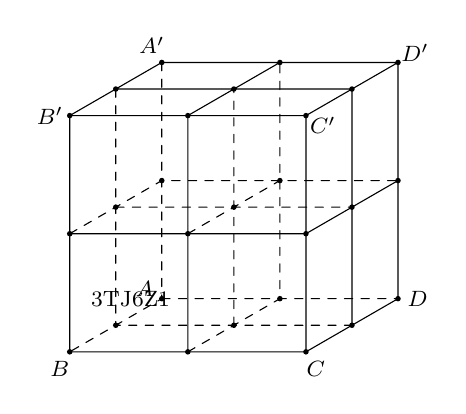
\begin{tikzpicture}[scale=1,>=stealth, font=\footnotesize, line join=round, line cap=round, declare function={h=3;}]
    %hidden: VM005
				\path
					(0,0) coordinate (A)
					(A)+(-150:0.45*h) coordinate (B)
					(B)+(0:h) coordinate (C)
					(barycentric cs:A=1,C=1,B=-1)coordinate(D)
					(A)+(90:h) coordinate (A')
					(barycentric cs:A=-1,B=1,A'=1)coordinate(B')
					(barycentric cs:A=-1,C=1,A'=1)coordinate(C')
					(barycentric cs:A=-1,D=1,A'=1)coordinate(D')
					;
				\foreach \x/\y/\t in{A/B/E,B/C/F,C/D/G,D/A/H,A/A'/M,B/B'/N,C/C'/P,D/D'/Q,A'/B'/E',B'/C'/F',C'/D'/G',D'/A'/H'}
				{\path (barycentric cs:\x=1,\y=1) coordinate(\t);}
				\foreach \x/\y/\t in{M/N/X,N/P/Y,P/Q/Z,Q/M/T,B/D/U,N/Q/V,B'/D'/W}
				{\path (barycentric cs:\x=1,\y=1)coordinate(\t);}
				\draw[dashed] (A')--(A)--(B) (A)--(D)
					(N)--(M)--(Q) (X)--(Z) (Y)--(T) (F)--(H)--(H') (U)--(W) (E')--(E)--(G)
					;
				\draw (D')--(A')--(B')--(B)--(C)--(D)--(D')--(C')--(B') (C)--(C')
					(N)--(P)--(Q) (F)--(F')--(H') (E')--(G')--(G);
				\foreach \p/\u in{A/150,B/-120,C/-60,D/0,A'/120,B'/180,C'/-30,D'/30}
				\fill(\p) circle(1pt) node[shift={(\u:.25)}]{$\p$};
				\foreach \p in{E,F,G,H,M,N,P,Q,E',F',G',H',X,Y,Z,T,U,V,W}
				\fill (\p) circle(1pt);
    \node at (0,0){\href{3TJ6Z1}{\tiny \phantom{3TJ6Z1}}};
			\end{tikzpicture}
		\end{center}
		\begin{itemize}
			\item \textbf{Bước 1:} Tổng số điểm (đỉnh của các khối lập phương cạnh $1$\,cm) là $3\cdot 3\cdot 3=27$ (điểm).
			\item \textbf{Bước 2:} Tổng số cách chọn $3$ điểm bất kỳ là $\mathrm{C}_{27}^3=2\,925$ (cách).
			\item \textbf{Bước 3:} Loại trừ các trường hợp $3$ điểm không tạo thành tam giác (ba điểm thẳng hàng).\\
			Các đường thẳng chứa $3$ điểm được chia thành $3$ trường hợp sau:
			\begin{enumerate}[\it TH 1:]
				\item Các đường thẳng song song với các cạnh của khối lập phương.
				\begin{itemize}
					\item Có $3$ hướng $\left(AB,AD,AA'\right)$.
					\item Mỗi hướng có $3\cdot 3=9$ đường thẳng (mỗi đường này gồm ba điểm thẳng hàng).
				\end{itemize}
				Số bộ ba điểm thẳng hàng là $3\cdot 9=27$ (bộ).
				\item Các đường thẳng song song với đường chéo của các mặt.
				\begin{itemize}
					\item Khối lập phương có $3$ hướng mặt phẳng $\left((ABCD),\left(ABB'A'\right),\left(ADD'A'\right)\right)$.
					\item Mỗi hướng có $3$ lớp mặt phẳng song song.
					\item Trên mỗi mặt phẳng có $2$ đường chéo chính chứa $3$ điểm.
				\end{itemize}
				Số bộ ba điểm thẳng hàng là $3\cdot 3\cdot 2=18$ (bộ).
				\item Các đường chéo đi qua tâm của khối lập phương lớn $\left(AC',BD',CA',DB'\right)$.\\
				Mỗi đường này chứa đúng $3$ điểm.\\
				Số bộ ba điểm thẳng hàng là $4$ (bộ).
			\end{enumerate}
			Tổng số bộ $3$ điểm thẳng hàng là $27+18+4=49$ (bộ).
			\item \textbf{Bước 4:} Tính số tam giác\\
			Số tam giác là $2\,925-49=2\,876$.
		\end{itemize}
		Vậy có $2\,876$ tam giác được tạo thành từ các đỉnh của các khối lập phương cạnh $1$\,cm.
	}
\end{ex}

\Closesolutionfile{ans}
\Closesolutionfile{ansbook}
\begin{indapan}
	{ans/ans\currfilebase}
\end{indapan}